% !TeX program = xelatex
\documentclass[11pt,a4paper,fontset=fandol]{ctexart}

% ============================ 1. 基础页面设置 ================================
\usepackage{geometry}
\geometry{left=2.5cm, right=2.5cm, top=2.5cm, bottom=2.5cm}

% ============================ 2. 数学基础包与标准定理 ========================
\usepackage{amsmath, amssymb, amsthm}
\usepackage{mathtools}
\usepackage{bm}                       % 向量/矩阵加粗
\allowdisplaybreaks                   % 长公式跨页

% 标准学术定理环境（除定义外，其余均直接在正文中排版，无多余框线）
\newtheorem{theorem}{定理}[section]
\newtheorem{lemma}[theorem]{引理}
\newtheorem{property}[theorem]{性质}
\newtheorem{corollary}[theorem]{推论}

\theoremstyle{remark}
\newtheorem{remark}{注}[section]

% ============================ 3. 字体设置 ====================================
\usepackage{newtxtext}               % 英文 Times 系列
\usepackage{newtxmath}               % 数学公式 Times 系列

% ============================ 4. 仅定义使用的独立环境 ========================
\usepackage[most]{tcolorbox}

% 定义环境：学术极简浅灰底+细边框（单独突出）
\newtcbtheorem[number within=section]{definition}{定义}{
    enhanced,
    boxrule=0.5pt,
    arc=0pt,
    colback=gray!4!white,
    colframe=black!80,
    fonttitle=\bfseries\sffamily,
    coltitle=black,
    attach boxed title to top left={yshift=-2mm, xshift=2mm},
    boxed title style={boxrule=0pt, colframe=white, colback=white},
    separator sign={\ },
    description font=\normalfont
}{def}

% ============================ 5. 图表与列表 ==================================
\usepackage{booktabs}
\usepackage{graphicx}
\usepackage{enumitem}
\setlist{nosep, leftmargin=2em}

\usepackage{caption}
\captionsetup{font=small, labelfont=bf, justification=centering}

% 绘图支持
\usepackage{tikz}
\usetikzlibrary{arrows.meta, positioning, calc, patterns}

% ============================ 6. 超链接设置 ==================================
\usepackage{hyperref}
\usepackage{cleveref}
\hypersetup{
    colorlinks=true,
    linkcolor=black,
    citecolor=black,
    urlcolor=black
}

% ============================ 7. 章节格式 ====================================
\ctexset{
    section/name={,},
    section/number=\arabic{section},
    section/format=\Large\bfseries,
    subsection/number=\arabic{section}.\arabic{subsection},
    subsection/format=\large\bfseries,
    subsubsection/number=\arabic{section}.\arabic{subsection}.\arabic{subsubsection},
    subsubsection/format=\normalsize\bfseries
}

\renewcommand{\baselinestretch}{1.15}
\setlength{\parskip}{0.3em}
\setlength{\parindent}{2em}

% ============================ 8. 页眉页脚 ====================================
\usepackage{fancyhdr}
\pagestyle{fancy}
\fancyhf{}
\fancyhead[L]{\small 复变函数}
\fancyhead[R]{\small \leftmark}
\fancyfoot[C]{\small\thepage}
\renewcommand{\headrulewidth}{0.4pt}

% ============================ 9. 正文开始 ====================================
\begin{document}

\section{复数与复变函数}

\subsection{复数及其代数运算}

\begin{definition}{复数}{complex_number}
形如 $z = x + iy$ 的数称为\textbf{复数}，其中 $x, y \in \mathbb{R}$，实数 $x$ 称为 $z$ 的\textbf{实部}，记作 $\operatorname{Re}(z) = x$；实数 $y$ 称为 $z$ 的\textbf{虚部}，记作 $\operatorname{Im}(z) = y$。符号 $i$ 称为\textbf{虚数单位}，满足基本关系式 $i^2 = -1$。
\end{definition}

对于任意整数 $k \in \mathbb{Z}$，虚数单位 $i$ 的正整数次幂呈现以 4 为周期的循环特性：
\begin{equation}
    i^{4k} = 1,\quad i^{4k+1} = i,\quad i^{4k+2} = -1,\quad i^{4k+3} = -i
\end{equation}

设两复数 $z_1 = x_1 + iy_1$ 与 $z_2 = x_2 + iy_2$，其基本代数运算法则如下：
\begin{enumerate}
    \item \textbf{相等}：$z_1 = z_2 \iff x_1 = x_2$ 且 $y_1 = y_2$。
    \item \textbf{加减法}：$z_1 \pm z_2 = (x_1 \pm x_2) + i(y_1 \pm y_2)$。
    \item \textbf{乘法}：$z_1 z_2 = (x_1 x_2 - y_1 y_2) + i(x_1 y_2 + x_2 y_1)$。
    \item \textbf{除法}（$z_2 \neq 0$）：
    \begin{equation}
        \frac{z_1}{z_2} = \frac{x_1 + iy_1}{x_2 + iy_2} = \frac{(x_1 x_2 + y_1 y_2) + i(x_2 y_1 - x_1 y_2)}{x_2^2 + y_2^2}
    \end{equation}
\end{enumerate}

\begin{definition}{共轭复数}{conjugate}
若 $z = x + iy$，则称 $\bar{z} = x - iy$ 为 $z$ 的\textbf{共轭复数}。
\end{definition}

\begin{property}[共轭运算基本性质]
共轭运算满足以下代数恒等关系：
\begin{align}
    \overline{z_1 \pm z_2} &= \bar{z}_1 \pm \bar{z}_2, &
    \overline{z_1 z_2} &= \bar{z}_1 \bar{z}_2, &
    \overline{\left(\frac{z_1}{z_2}\right)} &= \frac{\bar{z}_1}{\bar{z}_2} \quad (z_2 \neq 0) \\
    \operatorname{Re}(z) &= \frac{z + \bar{z}}{2}, &
    \operatorname{Im}(z) &= \frac{z - \bar{z}}{2i}, &
    z \bar{z} &= x^2 + y^2 = |z|^2
\end{align}
\end{property}

\subsection{复数的几何表示}

每个复数 $z = x + iy$ 唯一对应于平面直角坐标系中的点 $P(x,y)$，或以原点为起点的平面向量 $\overrightarrow{OP} = (x, y)$。建立该对应的几何平面称为\textbf{复平面}（或 Gauss 平面）。

\begin{figure}[htbp]
\centering
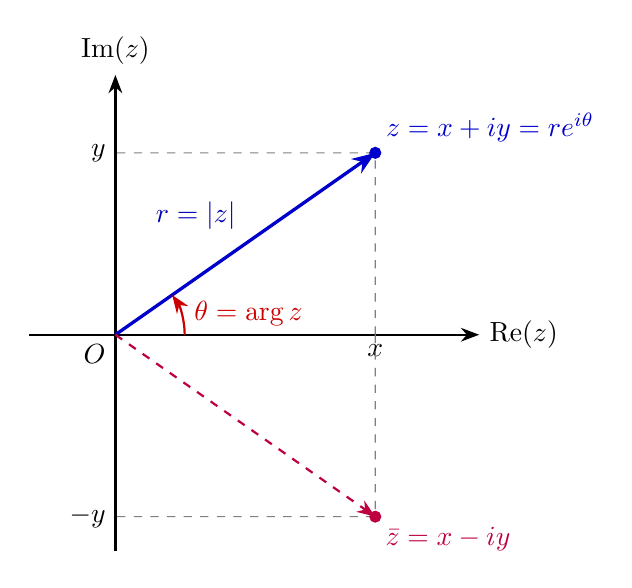
\begin{tikzpicture}[scale=1.1, >=Stealth]
    \draw[->, thick] (-1, 0) -- (4.2, 0) node[right] {$\operatorname{Re}(z)$};
    \draw[->, thick] (0, -2.5) -- (0, 3) node[above] {$\operatorname{Im}(z)$};
    \node[below left] at (0, 0) {$O$};

    % 点与向量 z
    \coordinate (Z) at (3, 2.1);
    \draw[->, very thick, blue!80!black] (0, 0) -- (Z) node[above right] {$z = x + iy = r e^{i\theta}$};
    \draw[dashed, gray] (3, 0) node[below, black] {$x$} -- (Z) -- (0, 2.1) node[left, black] {$y$};
    \filldraw[blue!80!black] (Z) circle (1.8pt);

    % 模与辐角
    \node[above left, blue!70!black] at (1.5, 1.1) {$r = |z|$};
    \draw[->, thick, red!80!black] (0.8, 0) arc (0:35:0.8);
    \node[right, red!80!black] at (0.8, 0.25) {$\theta = \arg z$};

    % 共轭点
    \coordinate (Zbar) at (3, -2.1);
    \draw[->, dashed, thick, purple] (0, 0) -- (Zbar) node[below right] {$\bar{z} = x - iy$};
    \draw[dashed, gray] (3, 0) -- (Zbar) -- (0, -2.1) node[left, black] {$-y$};
    \filldraw[purple] (Zbar) circle (1.8pt);
\end{tikzpicture}
\caption{复数的几何表示、极坐标分解与共轭对称}
\label{fig:complex_plane}
\end{figure}

\begin{definition}{模与辐角}{modulus_arg}
设 $z = x + iy$，实数 $r = \sqrt{x^2 + y^2}$ 称为 $z$ 的\textbf{模}（绝对值），记作 $|z|$。

对于非零复数 $z \neq 0$，向量 $\overrightarrow{OP}$ 与正实轴夹角 $\theta$ 称为 $z$ 的\textbf{辐角}，记作 $\operatorname{Arg} z$。辐角是多值函数：
\begin{equation}
    \operatorname{Arg} z = \arg z + 2k\pi \quad (k \in \mathbb{Z})
\end{equation}
其中满足区间 $-\pi < \arg z \le \pi$ 的唯一确定值称为\textbf{辐角主值}，记作 $\arg z$。
\end{definition}

辐角主值 $\arg z$ 由点 $(x, y)$ 所在象限确定：
\begin{equation}
    \arg z = \begin{cases}
        \arctan \dfrac{y}{x}, & x > 0, \\
        \arctan \dfrac{y}{x} + \pi, & x < 0, y \ge 0, \\
        \arctan \dfrac{y}{x} - \pi, & x < 0, y < 0, \\
        +\dfrac{\pi}{2}, & x = 0, y > 0, \\
        -\dfrac{\pi}{2}, & x = 0, y < 0.
    \end{cases}
\end{equation}

\begin{theorem}[三角不等式]
对任意复数 $z_1, z_2$，均有：
\begin{equation}
    \big| |z_1| - |z_2| \big| \le |z_1 \pm z_2| \le |z_1| + |z_2|
\end{equation}
\end{theorem}

由 Euler 公式 $e^{i\theta} = \cos\theta + i\sin\theta$，非零复数可表示为\textbf{三角形式}与\textbf{指数形式}：
\begin{equation}
    z = r(\cos\theta + i\sin\theta) = r e^{i\theta}
\end{equation}

\begin{theorem}[乘积与商的几何意义]
设 $z_1 = r_1 e^{i\theta_1}, z_2 = r_2 e^{i\theta_2}$，则：
\begin{equation}
    z_1 z_2 = r_1 r_2 e^{i(\theta_1 + \theta_2)}, \quad
    \frac{z_1}{z_2} = \frac{r_1}{r_2} e^{i(\theta_1 - \theta_2)} \quad (z_2 \neq 0)
\end{equation}
即：两复数相乘，模相乘，辐角相加；两复数相除，模相除，辐角相减。集合意义下有：
\begin{equation}
    \operatorname{Arg}(z_1 z_2) = \operatorname{Arg} z_1 + \operatorname{Arg} z_2, \quad
    \operatorname{Arg}\left(\frac{z_1}{z_2}\right) = \operatorname{Arg} z_1 - \operatorname{Arg} z_2
\end{equation}
\end{theorem}

\subsection{复数的乘幂与方根}

\begin{theorem}[De Moivre 公式]
对于任意整数 $n \in \mathbb{Z}$，恒有：
\begin{equation}
    (\cos\theta + i\sin\theta)^n = \cos(n\theta) + i\sin(n\theta) \iff (e^{i\theta})^n = e^{in\theta}
\end{equation}
\end{theorem}

\begin{definition}{复数的 $n$ 次方根}{root}
满足方程 $w^n = z$ 的复数 $w$ 称为 $z$ 的 $n$ 次方根，记为 $\sqrt[n]{z}$ 或 $z^{1/n}$。
\end{definition}

设非零复数 $z = r e^{i\theta} = r e^{i(\arg z + 2k\pi)}$，则 $\sqrt[n]{z}$ 恰有 $n$ 个互不相同的复数值：
\begin{equation}
    w_k = \sqrt[n]{r} \exp\left( i \frac{\arg z + 2k\pi}{n} \right), \quad k = 0, 1, 2, \dots, n-1
\end{equation}
在几何上，$w_k$ 的模全为 $\sqrt[n]{r}$，位于以原点为中心的圆周上，对应辐角逐次递增 $\frac{2\pi}{n}$，构成了圆内接正 $n$ 边形的全部顶点。

\begin{figure}[htbp]
\centering
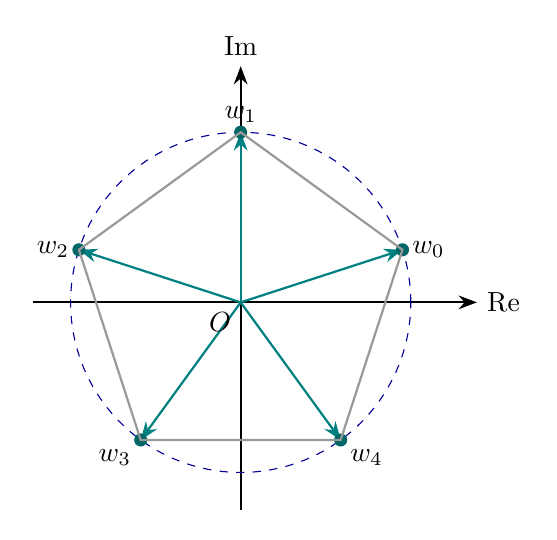
\begin{tikzpicture}[scale=1.2, >=Stealth]
    \draw[->, thick] (-2.2, 0) -- (2.5, 0) node[right] {$\operatorname{Re}$};
    \draw[->, thick] (0, -2.2) -- (0, 2.5) node[above] {$\operatorname{Im}$};
    \draw[dashed, blue!60!black] (0, 0) circle (1.8cm);

    \foreach \k in {0,1,2,3,4} {
        \coordinate (P\k) at ({1.8*cos(18 + \k*72)}, {1.8*sin(18 + \k*72)});
        \draw[->, thick, teal] (0, 0) -- (P\k);
        \filldraw[teal!80!black] (P\k) circle (1.8pt);
    }
    \draw[thick, gray!80] (P0) -- (P1) -- (P2) -- (P3) -- (P4) -- cycle;
    \node[right] at (P0) {$w_0$};
    \node[above] at (P1) {$w_1$};
    \node[left] at (P2) {$w_2$};
    \node[below left] at (P3) {$w_3$};
    \node[below right] at (P4) {$w_4$};
    \node[below left] at (0, 0) {$O$};
\end{tikzpicture}
\caption{复数开方根的几何构型（以 $n = 5$ 为例：均匀分布的正五边形顶点）}
\label{fig:roots}
\end{figure}

\subsection{平面点集与区域}

\begin{definition}{邻域与开集}{open_set}
\begin{enumerate}
    \item 设 $z_0 \in \mathbb{C}, \delta > 0$，点集 $U(z_0, \delta) = \{z \in \mathbb{C} \mid |z - z_0| < \delta\}$ 称为 $z_0$ 的\textbf{$\delta$ 邻域}；集合 $\mathring{U}(z_0, \delta) = \{z \in \mathbb{C} \mid 0 < |z - z_0| < \delta\}$ 称为 $z_0$ 的\textbf{去心 $\delta$ 邻域}。
    \item 设 $G \subset \mathbb{C}$ 为点集。若 $\forall z \in G$，存在 $\delta > 0$ 使得 $U(z, \delta) \subset G$，则称 $z$ 为 $G$ 的\textbf{内点}。若 $G$ 中所有的点都是内点，则称 $G$ 为\textbf{开集}。
\end{enumerate}
\end{definition}

\begin{definition}{区域与连通性}{domain}
\begin{enumerate}
    \item 平面点集 $D$ 称为一个\textbf{区域}，如果它满足：
    \begin{itemize}
        \item $D$ 是开集；
        \item $D$ 是连通的（即 $D$ 内任意两点均可用完全落在 $D$ 内部的有限折线连接）。
    \end{itemize}
    \item 若某点 $P$ 的任意邻域内既含有属于 $D$ 的点，又含有不属于 $D$ 的点，则称 $P$ 为 $D$ 的\textbf{边界点}。全体边界点的集合称为 $D$ 的\textbf{边界}，记作 $\partial D$。集合 $\bar{D} = D \cup \partial D$ 称为\textbf{闭区域}。
\end{enumerate}
\end{definition}

\begin{figure}[htbp]
\centering
\begin{tikzpicture}[scale=1.1, >=Stealth]
    % 单连通
    \begin{scope}[shift={(-3,0)}]
        \draw[thick, fill=blue!10, rounded corners=12pt] (-1.8, -1.2) rectangle (1.5, 1.3);
        \node at (0, 0) {$D_1$（单连通域）};
        \draw[thick, purple, ->] (-0.8, -0.6) to[out=40, in=140] (0.8, -0.6);
        \filldraw[purple] (-0.8, -0.6) circle (1.5pt) node[left] {$A$};
        \filldraw[purple] (0.8, -0.6) circle (1.5pt) node[right] {$B$};
    \end{scope}

    % 多连通
    \begin{scope}[shift={(3,0)}]
        \draw[thick, fill=orange!12, rounded corners=14pt] (-2, -1.4) rectangle (2, 1.4);
        \draw[thick, fill=white] (-0.7, 0.1) circle (0.55cm);
        \draw[thick, fill=white] (0.8, -0.2) circle (0.4cm);
        \node at (-0.7, 0.1) {$H_1$};
        \node at (0.8, -0.2) {$H_2$};
        \node at (0, 1.0) {$D_2$（多连通域）};
    \end{scope}
\end{tikzpicture}
\caption{单连通区域（无洞）与多连通区域（含空洞或多个互不连通边界）示意}
\label{fig:domain_connectivity}
\end{figure}

\begin{remark}
直观而言，若区域 $D$ 内任何闭合曲线的内部都完全属于 $D$（即区域内不含有“孔洞”），则称 $D$ 为\textbf{单连通区域}；反之，若区域内包含“孔洞”，则称为\textbf{多连通区域}。
\end{remark}

\subsection{复变函数的概念与几何映射}

\begin{definition}{复变函数与映射}{complex_function}
设 $D$ 为复平面上的点集。若按照某一对应法则 $f$，对于 $D$ 中的每一个复数 $z = x + iy$，都有一个或多个确定的复数 $w = u + iv$ 与之对应，则称 $w$ 为定义在 $D$ 上的\textbf{复变函数}，记作：
\begin{equation}
    w = f(z) = u(x, y) + i v(x, y)
\end{equation}
其中 $u(x, y)$ 和 $v(x, y)$ 是关于两个实自变量 $x, y$ 的实二元函数。

在几何上，复变函数建立了解析平面 $z$ 到映射平面 $w$ 的点集对应关系，称之为\textbf{几何变换}或\textbf{映射}。
\end{definition}

\begin{figure}[htbp]
\centering
\begin{tikzpicture}[scale=1.0, >=Stealth]
    % z 平面
    \draw[->] (-0.5, 0) -- (3, 0) node[right] {$x$};
    \draw[->] (0, -0.5) -- (0, 2.5) node[above] {$y$};
    \draw[thick, fill=cyan!15] (0.8, 0.6) to[out=20, in=190] (2.2, 1.0) to[out=70, in=330] (1.6, 2.0) to[out=170, in=80] (0.8, 0.6);
    \node at (1.5, 1.3) {$G \subset \mathbb{C}_z$};
    \filldraw[blue] (1.2, 1.0) circle (1.5pt) node[below] {$z$};
    \node at (1.2, -0.7) {$z\text{ 平面}$};

    % 映射箭头
    \draw[->, very thick, red!80!black] (3.4, 1.2) -- (4.8, 1.2) node[midway, above] {$w = f(z)$};

    % w 平面
    \begin{scope}[shift={(5.5,0)}]
        \draw[->] (-0.5, 0) -- (3, 0) node[right] {$u$};
        \draw[->] (0, -0.5) -- (0, 2.5) node[above] {$v$};
        \draw[thick, fill=purple!15] (1.0, 0.4) to[out=40, in=170] (2.4, 0.8) to[out=100, in=320] (1.9, 2.2) to[out=190, in=90] (1.0, 0.4);
        \node at (1.7, 1.3) {$G^* \subset \mathbb{C}_w$};
        \filldraw[purple] (1.4, 1.1) circle (1.5pt) node[below] {$w = f(z)$};
        \node at (1.2, -0.7) {$w\text{ 平面}$};
    \end{scope}
\end{tikzpicture}
\caption{复变函数作为复平面点集映射的几何机制}
\label{fig:mapping}
\end{figure}

常见初等映射的几何变换行为包括：
\begin{enumerate}
    \item \textbf{平移变换} $w = z + b$：将复平面上的图形沿向量 $(\operatorname{Re}(b), \operatorname{Im}(b))$ 刚性平移。
    \item \textbf{旋转变换} $w = e^{i\alpha} z$（$\alpha \in \mathbb{R}$）：绕原点逆时针旋转角度 $\alpha$。
    \item \textbf{伸缩变换} $w = k z$（$k > 0$）：以原点为中心进行比例为 $k$ 的均匀缩放。
    \item \textbf{旋转伸缩变换} $w = a z$（$a = R e^{i\alpha}$）：模放大 $R$ 倍，同时辐角逆时针旋转 $\alpha$。
    \item \textbf{幂映射} $w = z^2$：点 $z = r e^{i\theta} \mapsto w = r^2 e^{i 2\theta}$，使点到原点距离变为原来的平方，辐角扩大 2 倍（角形区域展宽）。
\end{enumerate}

\subsection{复变函数的极限与连续性}

\begin{definition}{函数极限}{limit}
设函数 $w = f(z)$ 定义在去心邻域 $\mathring{U}(z_0, \rho)$ 内，$A \in \mathbb{C}$ 为常数。若对于任意给定的 $\varepsilon > 0$，均存在 $\delta > 0$ ($0 < \delta < \rho$)，使得当 $0 < |z - z_0| < \delta$ 时，恒有：
\begin{equation}
    |f(z) - A| < \varepsilon
\end{equation}
则称常数 $A$ 为函数 $f(z)$ 当 $z \to z_0$ 时的\textbf{极限}，记作 $\lim_{z \to z_0} f(z) = A$。
\end{definition}

\begin{remark}
定义中 $z \to z_0$ 是指 $z$ 在复平面二维空间内\textbf{以任意方式、沿任意曲线路径}逼近 $z_0$。只要存在两条不同逼近路径导致极限值不同，则极限必不存在。
\end{remark}

\begin{theorem}[极限充要条件]
设 $f(z) = u(x, y) + i v(x, y)$，$z_0 = x_0 + i y_0$，$A = u_0 + i v_0$，则：
\begin{equation}
    \lim_{z \to z_0} f(z) = A \iff \lim_{\substack{x \to x_0 \\ y \to y_0}} u(x, y) = u_0 \quad \text{且} \quad \lim_{\substack{x \to x_0 \\ y \to y_0}} v(x, y) = v_0
\end{equation}
\end{theorem}

\begin{definition}{函数连续性}{continuous}
设函数 $w = f(z)$ 定义在区域 $D$ 内，$z_0 \in D$。若：
\begin{equation}
    \lim_{z \to z_0} f(z) = f(z_0)
\end{equation}
则称 $f(z)$ 在点 $z_0$ 处\textbf{连续}。若 $f(z)$ 在区域 $D$ 内每一点均连续，则称 $f(z)$ 在区域 $D$ 内连续。
\end{definition}

\begin{theorem}[连续充要条件与性质]
函数 $f(z) = u(x, y) + i v(x, y)$ 在 $z_0 = x_0 + iy_0$ 处连续的充分必要条件是其实部 $u(x, y)$ 与虚部 $v(x, y)$ 作为二元实函数在 $(x_0, y_0)$ 处均连续。连续复变函数的和、差、积、商（分母不为零）以及复合函数仍为连续函数。
\end{theorem}

\section{解析函数}

\subsection{解析函数的概念}

\begin{definition}{复变函数的导数与微分}{derivative}
设函数 $w = f(z)$ 定义于区域 $D$ 内，$z_0 \in D$。若极限
\begin{equation}
    f'(z_0) = \lim_{\Delta z \to 0} \frac{f(z_0 + \Delta z) - f(z_0)}{\Delta z} = \lim_{z \to z_0} \frac{f(z) - f(z_0)}{z - z_0}
\end{equation}
存在，则称 $f(z)$ 在点 $z_0$ 处\textbf{可导}（可微），该极限值称为 $f(z)$ 在 $z_0$ 处的\textbf{导数}，记作 $f'(z_0)$ 或 $\left.\frac{\mathrm{d}w}{\mathrm{d}z}\right|_{z = z_0}$。

若函数增量可表示为 $\Delta w = f'(z_0)\Delta z + o(|\Delta z|)$，则称 $\mathrm{d}w = f'(z_0)\mathrm{d}z$ 为 $f(z)$ 在点 $z_0$ 处的\textbf{微分}。复变函数在一点处可导与可微等价。
\end{definition}

\begin{definition}{解析函数与奇点}{analytic_function}
设函数 $f(z)$ 定义于平面点集 $G$ 上：
\begin{enumerate}
    \item 若 $f(z)$ 在点 $z_0$ 及其某个邻域 $U(z_0, \delta)$ 内处处可导，则称 $f(z)$ 在点 $z_0$ \textbf{解析}。
    \item 若 $f(z)$ 在区域 $D$ 内的每一点均解析（等价于在 $D$ 内处处可导），则称 $f(z)$ 为区域 $D$ 内的\textbf{解析函数}（全纯函数）。
    \item 若 $f(z)$ 在点 $z_0$ 处不可导（或不解析），但在 $z_0$ 的任一去心邻域内都包含解析点，则称 $z_0$ 为 $f(z)$ 的\textbf{奇点}。
\end{enumerate}
\end{definition}

\begin{figure}[htbp]
\centering
\begin{tikzpicture}[scale=0.95, >=Stealth, 
    box/.style={draw, rounded corners=3pt, align=center, font=\small, inner sep=6pt},
    arr/.style={->, thick}]
    
    % 第一行节点
    \node[box, fill=gray!8, text width=2.2cm] (cont) at (0, 0) {连续};
    \node[box, fill=cyan!12, text width=2.4cm] (ptdiff) at (4.6, 0) {在 $z_0$ 处可导};
    \node[box, fill=teal!15, text width=2.4cm] (ptana) at (9.2, 0) {在 $z_0$ 处解析};

    % 第二行节点
    \node[box, fill=blue!12, text width=3.0cm] (domdiff) at (4.6, -2.6) {在区域 $D$ 内\\处处可导};
    \node[box, fill=blue!18, text width=3.0cm] (domana) at (9.2, -2.6) {在区域 $D$ 内\\解析};

    % 单点关系连线（上下错开单向箭头，防止重叠）
    \draw[arr] ([yshift=3pt]ptdiff.west) -- ([yshift=3pt]cont.east) 
        node[midway, above=1pt, font=\footnotesize] {推出};
    \draw[arr, dashed, red!80!black] ([yshift=-3pt]cont.east) -- ([yshift=-3pt]ptdiff.west) 
        node[midway, below=1pt, font=\footnotesize] {推不出};

    \draw[arr] ([yshift=3pt]ptana.west) -- ([yshift=3pt]ptdiff.east) 
        node[midway, above=1pt, font=\footnotesize] {推出};
    \draw[arr, dashed, red!80!black] ([yshift=-3pt]ptdiff.east) -- ([yshift=-3pt]ptana.west) 
        node[midway, below=1pt, font=\footnotesize] {推不出};

    % 纵向与横向关联
    \draw[<->, double, thick, blue!80!black] (domdiff) -- (domana) 
        node[midway, above=2pt, font=\footnotesize] {等价};
    \draw[arr] ([xshift=10pt]domana.north) -- ([xshift=10pt]ptana.south) 
        node[midway, right=2pt, font=\footnotesize] {蕴含};
    \draw[arr] ([xshift=-10pt]domdiff.north) -- ([xshift=-10pt]ptdiff.south) 
        node[midway, left=2pt, font=\footnotesize] {蕴含};
\end{tikzpicture}
\caption{连续、可导、单点解析与区域解析的概念逻辑结构}
\label{fig:analytic_logic}
\end{figure}

\begin{remark}
复变函数在一点可导的条件远比实函数严格。复增量 $\Delta z = \Delta x + i\Delta y \to 0$ 是在二维平面内沿任意可能路径逼近原点，所有方向极限必须同时存在且唯一。

“在一点处可导”与“在一点处解析”并不等价：若函数仅在单独隔离点处可导（其任意邻域内其余点均不可导），则该函数在该点可导但\textbf{绝不解析}。典型反例为 $f(z) = |z|^2 = x^2 + y^2$，该函数仅在原点 $z = 0$ 处可导（$f'(0)=0$），而在复平面内任何邻域内处处不解析。
\end{remark}

\subsection{解析函数的充要条件（Cauchy-Riemann 方程）}

\begin{theorem}[Cauchy-Riemann 方程与可导必要条件]
设函数 $f(z) = u(x, y) + i v(x, y)$ 在点 $z = x + iy$ 处可导，则其实部 $u(x,y)$ 与虚部 $v(x,y)$ 在该点的偏导数必存在，且满足\textbf{Cauchy-Riemann 方程}（简记为 C-R 方程）：
\begin{equation}
    \frac{\partial u}{\partial x} = \frac{\partial v}{\partial y}, \qquad \frac{\partial u}{\partial y} = -\frac{\partial v}{\partial x}
\end{equation}
此时导数可表示为：
\begin{equation}
    f'(z) = \frac{\partial u}{\partial x} + i \frac{\partial v}{\partial x} = \frac{\partial v}{\partial y} - i \frac{\partial u}{\partial y} = \frac{\partial u}{\partial x} - i \frac{\partial u}{\partial y} = \frac{\partial v}{\partial y} + i \frac{\partial v}{\partial x}
\end{equation}
\end{theorem}

\begin{figure}[htbp]
\centering
\begin{tikzpicture}[scale=1.1, >=Stealth]
    % 坐标轴
    \draw[->, thick] (-0.8, 0) -- (5.2, 0) node[right] {$\Delta x$};
    \draw[->, thick] (0, -0.8) -- (0, 4.0) node[above] {$\Delta y$};
    \node[below left=2pt] at (0, 0) {$O$};

    % 沿实轴逼近
    \coordinate (Px) at (3.8, 0);
    \draw[->, line width=1.6pt, blue!85!black] (Px) -- (1.2, 0);
    \filldraw[blue!85!black] (Px) circle (2pt);
    \node[draw=blue!40, rounded corners=2pt, fill=white, inner sep=3pt, font=\small, align=center] 
        at (3.2, -1.0) {沿实轴逼近 ($\Delta y = 0$)\\导数极限为 $u_x + i v_x$};
    \draw[->, gray!70] (2.8, -0.55) -- (2.5, -0.08);

    % 沿虚轴逼近
    \coordinate (Py) at (0, 3.2);
    \draw[->, line width=1.6pt, red!85!black] (Py) -- (0, 1.0);
    \filldraw[red!85!black] (Py) circle (2pt);
    \node[draw=red!40, rounded corners=2pt, fill=white, inner sep=3pt, font=\small, align=right] 
        at (-1.8, 2.2) {沿虚轴逼近 ($\Delta x = 0$)\\导数极限为 $v_y - i u_y$};
    \draw[->, gray!70] (-0.4, 2.2) -- (-0.08, 2.2);

    % 任意方向逼近
    \draw[dashed, gray!70, line width=0.8pt] (3.6, 2.7) -- (0, 0);
    \draw[->, thick, gray!80] (2.4, 1.8) -- (1.2, 0.9);
    \node[draw=gray!50, rounded corners=2pt, fill=white, inner sep=3pt, font=\footnotesize, align=center] 
        at (3.8, 2.0) {任意路径逼近\\极限必须一致};
\end{tikzpicture}
\caption{C-R 方程的几何直观来源：实轴与虚轴逼近所得极限必须相等}
\label{fig:cr_derivation}
\end{figure}

\begin{theorem}[函数解析的充要条件]
设函数 $f(z) = u(x, y) + i v(x, y)$ 定义于区域 $D$ 内：
\begin{enumerate}
    \item \textbf{一点可导的充要条件}：$f(z)$ 在点 $z_0 = x_0 + iy_0$ 处可导 $\iff u(x, y)$ 与 $v(x, y)$ 在点 $(x_0, y_0)$ 处\textbf{可微}，且满足 C-R 方程。
    \item \textbf{区域解析的充要条件}：$f(z)$ 在区域 $D$ 内解析 $\iff u(x, y)$ 与 $v(x, y)$ 在 $D$ 内具有一阶\textbf{连续偏导数}，且满足 C-R 方程。
\end{enumerate}
\end{theorem}

\begin{property}[形式微商形式]
引入形式微分算子：
\begin{equation}
    \frac{\partial}{\partial z} = \frac{1}{2}\left(\frac{\partial}{\partial x} - i\frac{\partial}{\partial y}\right), \qquad \frac{\partial}{\partial \bar{z}} = \frac{1}{2}\left(\frac{\partial}{\partial x} + i\frac{\partial}{\partial y}\right)
\end{equation}
则 C-R 方程等价于：
\begin{equation}
    \frac{\partial f}{\partial \bar{z}} = \frac{1}{2}\left[ \left(\frac{\partial u}{\partial x} - \frac{\partial v}{\partial y}\right) + i\left(\frac{\partial v}{\partial x} + \frac{\partial u}{\partial y}\right) \right] = 0
\end{equation}
该恒等式深刻表明：\textbf{解析函数在形式上是不含 $\bar{z}$、仅依赖于单变量 $z$ 的函数}。例如 $f(z) = \bar{z}$ 由于 $\frac{\partial f}{\partial \bar{z}} = 1 \neq 0$，在复平面内处处不可导。
\end{property}

\begin{corollary}[解析函数的刚性性质]
若 $f(z)$ 在区域 $D$ 内解析，且满足下列条件之一，则 $f(z)$ 在 $D$ 内必恒为常数：
\begin{enumerate}
    \item $f'(z) \equiv 0$；
    \item 实部 $u(x, y)$ 恒为常数，或虚部 $v(x, y)$ 恒为常数；
    \item 模 $|f(z)|$ 恒为常数；
    \item 辐角 $\arg f(z)$ 恒为常数；
    \item 共轭函数 $\overline{f(z)}$ 在 $D$ 内亦解析。
\end{enumerate}
\end{corollary}

\subsection{初等函数及其解析性}

\begin{definition}{复指数函数}{exp_func}
对任意复数 $z = x + iy$，定义指数函数为：
\begin{equation}
    e^z = \exp(z) = e^x(\cos y + i\sin y)
\end{equation}
\end{definition}

\begin{property}[指数函数的性质]
\begin{enumerate}
    \item \textbf{整函数性}：$e^z$ 在全复平面 $\mathbb{C}$ 内处处解析，且 $(e^z)' = e^z$。
    \item \textbf{模与辐角}：$|e^z| = e^x = e^{\operatorname{Re}(z)} > 0$（故 $e^z \neq 0$ 恒成立），$\operatorname{Arg}(e^z) = y + 2k\pi$。
    \item \textbf{指数律与周期性}：$e^{z_1 + z_2} = e^{z_1}e^{z_2}$，且具有纯虚数周期 $T = 2\pi i$，即 $e^{z + 2k\pi i} = e^z$ ($k \in \mathbb{Z}$)。
\end{enumerate}
\end{property}

\begin{definition}{复对数函数}{log_func}
若 $e^w = z$ ($z \neq 0$)，则称 $w$ 为 $z$ 的对数，记作 $w = \operatorname{Ln} z$。对数函数为无限多值函数：
\begin{equation}
    \operatorname{Ln} z = \ln|z| + i\operatorname{Arg} z = \ln|z| + i(\arg z + 2k\pi), \quad k \in \mathbb{Z}
\end{equation}
当 $k = 0$ 时，称 $\ln z = \ln|z| + i\arg z$（$-\pi < \arg z \le \pi$）为\textbf{对数主值}。
\end{definition}

\begin{figure}[htbp]
\centering
\begin{tikzpicture}[scale=1.05, >=Stealth]
    % 割破平面底色
    \fill[blue!4] (-3.8, -2.4) rectangle (4.2, 2.4);

    % 坐标轴
    \draw[->, thick] (-4.0, 0) -- (4.4, 0) node[right] {$\operatorname{Re}$};
    \draw[->, thick] (0, -2.5) -- (0, 2.6) node[above] {$\operatorname{Im}$};

    % 割线与分支点
    \draw[line width=2.4pt, red!85!black] (-3.8, 0) -- (0, 0);
    \filldraw[black] (0, 0) circle (2.2pt);
    \node[below right=3pt, font=\small] at (0, 0) {$O$ (分支点)};

    % 割线标签（紧凑放置在割线左上部）
    \node[draw=red!60, rounded corners=2pt, fill=white, font=\small, inner sep=3pt] 
        at (-2.6, 1.8) {分支割线 $(-\infty, 0]$};
    \draw[->, gray!70] (-2.6, 1.5) -- (-2.6, 0.15);

    % 上侧逼近（箭头位于 x = -0.7，文字全部靠左排布，远离虚轴与右侧方框）
    \draw[->, thick, blue!85!black] (-0.7, 1.3) -- (-0.7, 0.25);
    \node[left=3pt, blue!85!black, font=\footnotesize, fill=white, inner sep=1.5pt] 
        at (-0.7, 0.75) {上侧逼近: $\operatorname{Im}(\ln z) \to +\pi$};

    % 下侧逼近（箭头位于 x = -0.7，文字靠左排布）
    \draw[->, thick, purple!85!black] (-0.7, -1.3) -- (-0.7, -0.25);
    \node[left=3pt, purple!85!black, font=\footnotesize, fill=white, inner sep=1.5pt] 
        at (-0.7, -0.75) {下侧逼近: $\operatorname{Im}(\ln z) \to -\pi$};

    % 右侧说明框（右移至 x = 2.4 开阔区，不越过虚轴）
    \node[draw=gray!50, rounded corners=3pt, fill=white, font=\footnotesize, align=center, inner sep=4pt] 
        at (2.4, 1.4) {割破平面 \\ $\mathbb{C} \setminus (-\infty, 0]$ \\ 内主值分支单值解析};
\end{tikzpicture}
\caption{对数主值分支 $\ln z$ 的分支割线与跃变边界}
\label{fig:branch_cut}
\end{figure}

\begin{theorem}[对数函数的单值分支解析性]
将复平面沿负实轴及原点割开，得到割破平面 $D = \mathbb{C} \setminus (-\infty, 0]$。在 $D$ 内，对数主值分支 $\ln z$ 为单值连续解析函数，且导数为：
\begin{equation}
    (\ln z)' = \frac{1}{z}
\end{equation}
\end{theorem}

\begin{definition}{一般幂函数与复三角函数}{power_trig}
\begin{enumerate}
    \item 设 $a \in \mathbb{C}$，定义一般幂函数为 $z^a = e^{a \operatorname{Ln} z}$（一般为多值函数）。
    \item 复三角函数由 Euler 公式延拓定义为：
    \begin{equation}
        \sin z = \frac{e^{iz} - e^{-iz}}{2i}, \qquad \cos z = \frac{e^{iz} + e^{-iz}}{2}
    \end{equation}
\end{enumerate}
\end{definition}

\begin{property}[复三角函数的特性]
复三角函数在全复平面上处处解析，微积分公式 $(\sin z)' = \cos z, (\cos z)' = -\sin z$ 仍旧成立，且仍具有实周期 $2\pi$。但与实函数存在本质差异：
\begin{enumerate}
    \item \textbf{无界性}：在复平面上 $\sin z$ 与 $\cos z$ 不再有界。例如当 $z = iy$ ($y \in \mathbb{R}$) 时，$\cos(iy) = \cosh y = \frac{e^y + e^{-y}}{2} \to +\infty$ ($y \to \infty$)。
    \item \textbf{零点一致性}：$\sin z = 0 \iff z = k\pi$；$\cos z = 0 \iff z = k\pi + \frac{\pi}{2}$ ($k \in \mathbb{Z}$)，复零点全部位于实轴上。
\end{enumerate}
\end{property}

\subsection{调和函数与共轭调和函数}

\begin{definition}{调和函数与共轭调和函数}{harmonic_function}
设二元实函数 $\varphi(x, y)$ 在区域 $D$ 内具有二阶连续偏导数，且满足 Laplace 方程：
\begin{equation}
    \Delta \varphi = \frac{\partial^2 \varphi}{\partial x^2} + \frac{\partial^2 \varphi}{\partial y^2} = 0
\end{equation}
则称 $\varphi(x, y)$ 为区域 $D$ 内的\textbf{调和函数}。

若实二元函数 $u(x, y)$ 与 $v(x, y)$ 在区域 $D$ 内均为调和函数，且满足 C-R 方程 $u_x = v_y, u_y = -v_x$，则称 $v(x, y)$ 为 $u(x, y)$ 的\textbf{共轭调和函数}。
\end{definition}

\begin{theorem}[解析函数与调和函数的关系]
\begin{enumerate}
    \item 若函数 $f(z) = u(x, y) + i v(x, y)$ 在区域 $D$ 内解析，则其实部 $u$ 和虚部 $v$ 均为 $D$ 内的调和函数，且 $v$ 是 $u$ 的共轭调和函数。
    \item 设区域 $D$ 为单连通域，若 $u(x, y)$ 为 $D$ 内的调和函数，则必存在 $u$ 的共轭调和函数 $v(x, y)$，使得 $f(z) = u + iv$ 在 $D$ 内解析，且 $v$ 在差一个实常数的意义下唯一确定。
\end{enumerate}
\end{theorem}

\begin{remark}
共轭调和关系具有\textbf{严格的单向次序性}：若 $v$ 是 $u$ 的共轭调和函数（即 $u + iv$ 解析），则 $u$ 通常\textbf{不是} $v$ 的共轭调和函数（因为 $v + iu = i(u - iv) = i\overline{f(z)}$ 一般不解析）。事实上，$u$ 的共轭调和函数是 $-v$。
\end{remark}

已知单连通域内的调和实部 $u(x, y)$，求共轭虚部 $v(x, y)$ 的常用方法：
\begin{enumerate}
    \item \textbf{全微分线积分法}：由于 $\mathrm{d}v = -u_y\,\mathrm{d}x + u_x\,\mathrm{d}y$ 为全微分，取基准点 $(x_0, y_0) \in D$：
    \begin{equation}
        v(x, y) = \int_{(x_0, y_0)}^{(x, y)} -u_y\,\mathrm{d}x + u_x\,\mathrm{d}y + C
    \end{equation}
    \item \textbf{不定积分法}：由 $v_y = u_x$ 对 $y$ 积分得 $v(x, y) = \int u_x\,\mathrm{d}y + g(x)$，再利用 $v_x = -u_y$ 确定待定函数 $g(x)$。
\end{enumerate}

\section{复变函数的积分}

\subsection{复变函数积分的概念与性质}

\begin{definition}{复变函数的积分}{complex_integral}
设 $C$ 为复平面上一条按段光滑的有向曲线，起点为 $A$，终点为 $B$。函数 $f(z)$ 定义在 $C$ 上。
顺着 $C$ 的方向，在曲线上任意插入分点 $A = z_0, z_1, \dots, z_{n-1}, z_n = B$ 将曲线分割为 $n$ 个小弧段，在每个小弧段 $z_{k-1}z_k$ 上任取一点 $\zeta_k$，作和式：
\begin{equation}
    S_n = \sum_{k=1}^n f(\zeta_k)\Delta z_k, \qquad (\Delta z_k = z_k - z_{k-1})
\end{equation}
记 $\lambda = \max_{1 \le k \le n} |\Delta z_k|$。若极限 $\lim_{\lambda \to 0} S_n$ 存在，且与曲线分割方式及分点选法无关，则称该极限为函数 $f(z)$ 沿有向曲线 $C$ 的\textbf{积分}，记作：
\begin{equation}
    \int_C f(z)\,\mathrm{d}z = \lim_{\lambda \to 0} \sum_{k=1}^n f(\zeta_k)\Delta z_k
\end{equation}
\end{definition}

\begin{figure}[htbp]
\centering
\begin{tikzpicture}[scale=1.1, >=Stealth]
    % 曲线 C 路径
    \draw[thick, blue!80!black] (0, 0) to[out=60, in=190] (2.2, 1.8) to[out=10, in=170] (5.2, 1.4);
    
    % 起点与终点
    \filldraw[black] (0, 0) circle (2pt) node[below left=2pt] {$A = z_0$};
    \filldraw[black] (5.2, 1.4) circle (2pt) node[right=3pt] {$B = z_n$};
    
    % 方向箭头与曲线名称
    \draw[->, very thick, blue!85!black] (1.0, 1.05) -- (1.2, 1.25);
    \node[above=2pt, blue!80!black] at (1.1, 1.35) {$C$};
    
    % 分点
    \coordinate (Zkminus1) at (2.2, 1.8);
    \coordinate (Zk) at (3.6, 1.72);
    \coordinate (Zeta) at (2.9, 1.88);
    
    \filldraw[teal!80!black] (Zkminus1) circle (1.8pt);
    \node[below=4pt, teal!80!black, font=\small] at (Zkminus1) {$z_{k-1}$};
    
    \filldraw[teal!80!black] (Zk) circle (1.8pt);
    \node[below=4pt, teal!80!black, font=\small] at (Zk) {$z_k$};
    
    \filldraw[red!80!black] (Zeta) circle (1.8pt);
    \node[draw=red!50, rounded corners=2pt, fill=white, inner sep=2pt, font=\footnotesize] 
        at (2.9, 2.6) {介值点 $\zeta_k \in \widehat{z_{k-1}z_k}$};
    \draw[->, gray!70] (2.9, 2.3) -- (Zeta);
    
    % 弦向量 Delta z_k
    \draw[->, thick, purple] (Zkminus1) -- (Zk);
    \node[below=2pt, purple, font=\footnotesize] at (2.9, 1.55) {$\Delta z_k = z_k - z_{k-1}$};
\end{tikzpicture}
\caption{复变函数线积分的和式定义与弦向量微元}
\label{fig:complex_integral_def}
\end{figure}

\begin{theorem}[积分的计算法]
设 $f(z) = u(x, y) + i v(x, y)$ 在按段光滑曲线 $C$ 上连续：
\begin{enumerate}
    \item \textbf{化为两个二元实变函数的第二类线积分}：
    \begin{equation}
        \int_C f(z)\,\mathrm{d}z = \int_C (u\,\mathrm{d}x - v\,\mathrm{d}y) + i \int_C (v\,\mathrm{d}x + u\,\mathrm{d}y)
    \end{equation}
    \item \textbf{参数方程代入法}：若曲线 $C$ 的参数方程为 $z = z(t) = x(t) + i y(t)$（$t$ 从 $\alpha$ 变化到 $\beta$），且 $z'(t)$ 在积分区间上连续，则：
    \begin{equation}
        \int_C f(z)\,\mathrm{d}z = \int_\alpha^\beta f\big(z(t)\big) z'(t)\,\mathrm{d}t
    \end{equation}
\end{enumerate}
\end{theorem}

\begin{property}[复积分的基本性质]
\begin{enumerate}
    \item $\int_{C^-} f(z)\,\mathrm{d}z = -\int_C f(z)\,\mathrm{d}z$；
    \item $\int_C \big[\alpha f(z) + \beta g(z)\big]\,\mathrm{d}z = \alpha \int_C f(z)\,\mathrm{d}z + \beta \int_C g(z)\,\mathrm{d}z$；
    \item 若 $C = C_1 + C_2$，则 $\int_C f(z)\,\mathrm{d}z = \int_{C_1} f(z)\,\mathrm{d}z + \int_{C_2} f(z)\,\mathrm{d}z$；
    \item \textbf{估值不等式（$ML$ 不等式）}：设曲线 $C$ 的弧长为 $L$。若沿 $C$ 满足 $|f(z)| \le M$，则：
    \begin{equation}
        \left| \int_C f(z)\,\mathrm{d}z \right| \le \int_C |f(z)|\,|\mathrm{d}z| \le M \cdot L
    \end{equation}
\end{enumerate}
\end{property}

\begin{theorem}[标准圆周基准积分公式]
设 $C$ 为以 $z_0$ 为中心、半径为 $r > 0$ 的正向（逆时针）圆周，对任意整数 $n \in \mathbb{Z}$，恒有：
\begin{equation}
    \oint_C (z - z_0)^n\,\mathrm{d}z = \begin{cases}
        2\pi i, & n = -1, \\
        0, & n \neq -1.
    \end{cases}
\end{equation}
该结果与圆心 $z_0$ 的位置以及圆周半径 $r$ 的大小完全无关。
\end{theorem}

\subsection{柯西—古萨（Cauchy-Goursat）基本定理}

\begin{theorem}[柯西—古萨定理（单连通域）]
设函数 $f(z)$ 在单连通区域 $D$ 内解析，则沿 $D$ 内任意一条闭曲线 $C$，积分恒为零：
\begin{equation}
    \oint_C f(z)\,\mathrm{d}z = 0
\end{equation}
\end{theorem}

\begin{remark}
若进一步要求导数 $f'(z)$ 连续，则由 Green 公式及 C-R 方程可直接给出初等证明：
\begin{align}
    \oint_C f(z)\,\mathrm{d}z &= \oint_C (u\,\mathrm{d}x - v\,\mathrm{d}y) + i \oint_C (v\,\mathrm{d}x + u\,\mathrm{d}y) \\
    &= \iint_G \left(-\frac{\partial v}{\partial x} - \frac{\partial u}{\partial y}\right)\mathrm{d}x\mathrm{d}y + i \iint_G \left(\frac{\partial u}{\partial x} - \frac{\partial v}{\partial y}\right)\mathrm{d}x\mathrm{d}y = 0
\end{align}
古萨的重大理论贡献在于：完全去除了对导数 $f'(z)$ 连续性的预设假设，仅凭解析性（即一阶复导数的存在性）即可严格证明该定理。
\end{remark}

\subsection{复合闭路定理与闭路变形原理}

\begin{theorem}[复合闭路定理（多连通域推广）]
设多连通区域 $D$ 的外边界为正向简单闭曲线 $C$，内部包含 $n$ 条互不相交且互不包含的正向简单闭曲线 $C_1, C_2, \dots, C_n$。若函数 $f(z)$ 在以 $C$ 及 $C_1^-, C_2^-, \dots, C_n^-$ 为边界的闭区域 $\bar{D}$ 上解析，则：
\begin{equation}
    \oint_C f(z)\,\mathrm{d}z = \sum_{k=1}^n \oint_{C_k} f(z)\,\mathrm{d}z
\end{equation}
即由外边界正向与各内边界负向构成的复合闭路 $\Gamma = C + C_1^- + \dots + C_n^-$ 满足 $\oint_\Gamma f(z)\,\mathrm{d}z = 0$。
\end{theorem}

\begin{figure}[htbp]
\centering
\begin{tikzpicture}[scale=1.1, >=Stealth]
    % 区域底色
    \draw[thick, fill=blue!6, rounded corners=18pt] (-3.4, -1.8) rectangle (3.4, 1.8);
    
    % 外边界 C 与正向指示
    \node[above=2pt, blue!85!black, font=\bfseries] at (0, 1.8) {$C$ (外边界)};
    \draw[->, line width=1.4pt, blue!85!black] (-0.3, 1.8) -- (0.3, 1.8);
    
    % 内孔洞 C1
    \filldraw[fill=white, draw=black, thick] (-1.6, 0) circle (0.85cm);
    \draw[->, line width=1.3pt, red!85!black] (-1.6, 0.85) -- (-1.85, 0.82);
    \node[font=\small] at (-1.6, 0) {$C_1$};
    
    % 内孔洞 C2
    \filldraw[fill=white, draw=black, thick] (1.6, 0) circle (0.75cm);
    \draw[->, line width=1.3pt, red!85!black] (1.6, 0.75) -- (1.35, 0.72);
    \node[font=\small] at (1.6, 0) {$C_2$};
    
    % 割线（辅助开缝）
    \draw[thick, dashed, gray!80] (-3.4, 0) -- (-2.45, 0);
    \draw[thick, dashed, gray!80] (2.35, 0) -- (3.4, 0);
\end{tikzpicture}
\caption{多连通区域的复合闭路剪开与积分等价转换（引入割线消除内部孔洞后，复合闭路上积分总和为零，即 $\oint_C f(z)\,\mathrm{d}z = \sum_{k=1}^n \oint_{C_k} f(z)\,\mathrm{d}z$）}
\label{fig:multiconnected_contour}
\end{figure}

\begin{corollary}[闭路变形原理]
一个在区域内解析的函数沿闭曲线的积分，不因闭曲线在区域内作连续变形而改变其值，只要在变形过程中闭曲线不经过函数的奇点。
\end{corollary}

\subsection{原函数与不定积分}

\begin{theorem}[积分与路径无关性]
若函数 $f(z)$ 在单连通区域 $D$ 内解析，则积分 $\int_C f(z)\,\mathrm{d}z$ 仅与起点 $z_1$ 和终点 $z_2$ 有关，而与连接这两点的具体路径无关，记为 $\int_{z_1}^{z_2} f(z)\,\mathrm{d}z$。
\end{theorem}

\begin{theorem}[变上限积分与原函数存在性]
设 $f(z)$ 在单连通区域 $D$ 内解析，$z_0 \in D$ 为固定基准点。则变上限积分
\begin{equation}
    F(z) = \int_{z_0}^z f(\zeta)\,\mathrm{d}\zeta
\end{equation}
在 $D$ 内处处解析，且满足：
\begin{equation}
    F'(z) = f(z)
\end{equation}
即解析函数必有原函数。若 $\Phi(z)$ 满足 $\Phi'(z) = f(z)$，则 $\Phi(z)$ 称为 $f(z)$ 的原函数，且成立 \textbf{Newton-Leibniz 公式}：
\begin{equation}
    \int_{z_1}^{z_2} f(z)\,\mathrm{d}z = \Phi(z_2) - \Phi(z_1)
\end{equation}
\end{theorem}

\subsection{柯西积分公式}

\begin{theorem}[柯西积分公式]
设区域 $D$ 的边界为简单正向闭曲线 $C$。若函数 $f(z)$ 在 $D$ 内解析，在闭区域 $\bar{D} = D \cup C$ 上连续，则对 $D$ 内任意一点 $z_0$，恒有：
\begin{equation}
    f(z_0) = \frac{1}{2\pi i} \oint_C \frac{f(z)}{z - z_0}\,\mathrm{d}z
\end{equation}
\end{theorem}

\begin{figure}[htbp]
\centering
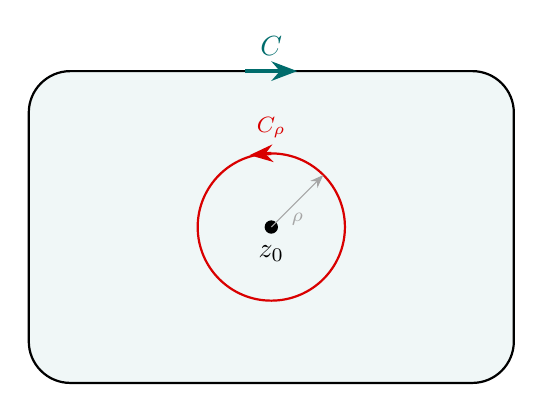
\begin{tikzpicture}[scale=1.1, >=Stealth]
    % 闭区域 D 轮廓
    \draw[thick, fill=teal!6, rounded corners=15pt] (-2.8, -1.8) rectangle (2.8, 1.8);
    \node[above=2pt, teal!85!black, font=\bfseries] at (0, 1.8) {$C$};
    \draw[->, line width=1.4pt, teal!85!black] (-0.3, 1.8) -- (0.3, 1.8);
    
    % 内部点 z_0 与小圆周 C_\rho
    \coordinate (Z0) at (0, 0);
    \filldraw[black] (Z0) circle (2pt) node[below=3pt] {$z_0$};
    
    \draw[thick, red!85!black] (Z0) circle (0.85cm);
    \draw[->, line width=1.2pt, red!85!black] (0, 0.85) -- (-0.25, 0.83);
    \node[above=2pt, red!85!black, font=\footnotesize] at (0, 0.85) {$C_\rho$};
    \draw[->, gray!70] (Z0) -- (0.6, 0.6) node[midway, below=1pt, font=\scriptsize] {$\rho$};
\end{tikzpicture}
\caption{柯西积分公式原理：外边界 $C$ 积分全息决定内部任意点 $z_0$ 函数值；通过复合闭路将外边界缩紧至以 $z_0$ 为中心的小圆周 $C_\rho$，当 $\rho \to 0$ 时取极限得出 $f(z_0) = \frac{1}{2\pi i}\oint_C \frac{f(z)}{z - z_0}\,\mathrm{d}z$}
\label{fig:cauchy_integral_formula}
\end{figure}

\begin{corollary}[平均值定理]
若 $f(z)$ 在闭圆盘 $|z - z_0| \le R$ 上解析，取积分回路为圆周 $z = z_0 + R e^{i\theta}$，则由柯西积分公式可得：
\begin{equation}
    f(z_0) = \frac{1}{2\pi} \int_0^{2\pi} f(z_0 + R e^{i\theta})\,\mathrm{d}\theta
\end{equation}
即解析函数在圆心处的值等于它在圆周边界上各点函数值的算术平均值。
\end{corollary}

\subsection{解析函数的高阶导数公式}

\begin{theorem}[高阶导数公式]
设函数 $f(z)$ 在正向简单闭曲线 $C$ 所围区域 $D$ 内解析，在闭区域 $\bar{D}$ 上连续，则 $f(z)$ 在 $D$ 内具有任意阶导数，且任意 $n$ 阶导数仍为 $D$ 内的解析函数。其表达式为：
\begin{equation}
    f^{(n)}(z_0) = \frac{n!}{2\pi i} \oint_C \frac{f(z)}{(z - z_0)^{n+1}}\,\mathrm{d}z \qquad (n = 1, 2, 3, \dots)
\end{equation}
\end{theorem}

\begin{remark}
高阶导数公式的主要计算作用是\textbf{通过求导来快速计算某些复变函数的闭路围道积分}：
\begin{equation}
    \oint_C \frac{f(z)}{(z - z_0)^{n+1}}\,\mathrm{d}z = \frac{2\pi i}{n!} f^{(n)}(z_0)
\end{equation}
\end{remark}

\begin{theorem}[柯西不等式与 Liouville 定理]
\begin{enumerate}
    \item \textbf{柯西不等式}：若 $f(z)$ 在 $|z - z_0| \le R$ 上解析且 $|f(z)| \le M$，则对任意正整数 $n$ 均有：
    \begin{equation}
        |f^{(n)}(z_0)| \le \frac{n! M}{R^n}
    \end{equation}
    \item \textbf{Liouville 定理}：在全复平面上解析且有界的整函数必恒为常数。
    \item \textbf{代数基本定理}：在复数域中，任何次数 $n \ge 1$ 的复系数多项式方程 $P_n(z) = a_n z^n + \dots + a_1 z + a_0 = 0$ ($a_n \neq 0$) 至少有一个复根。
\end{enumerate}
\end{theorem}

\subsection{解析函数与调和函数的关系}

\begin{theorem}[解析性对调和性的深化]
若函数 $f(z) = u(x, y) + i v(x, y)$ 在区域 $D$ 内解析，则由解析函数具有任意阶导数这一性质可知：实部 $u(x, y)$ 与虚部 $v(x, y)$ 在 $D$ 内均具有\textbf{任意阶连续偏导数}。特别地，各二阶混合偏导数均与求导次序无关，二者必满足 Laplace 方程：
\begin{equation}
    \frac{\partial^2 u}{\partial x^2} + \frac{\partial^2 u}{\partial y^2} = 0, \qquad \frac{\partial^2 v}{\partial x^2} + \frac{\partial^2 v}{\partial y^2} = 0
\end{equation}
因此解析函数的实部与虚部必为调和函数，且 $v$ 是 $u$ 的共轭调和函数。
\end{theorem}

\begin{remark}
在单连通域中，由调和实部 $u(x, y)$ 求解共轭虚部 $v(x, y)$ 时，微分式
\begin{equation}
    \mathrm{d}v = -u_y\,\mathrm{d}x + u_x\,\mathrm{d}y
\end{equation}
的回路积分沿任何闭曲线均恒为零，因此线积分
\begin{equation}
    v(x, y) = \int_{(x_0, y_0)}^{(x, y)} -u_y\,\mathrm{d}x + u_x\,\mathrm{d}y + C
\end{equation}
的取值与所选积分路线完全无关。
\end{remark}

\section{级数}

\subsection{复数项级数}

\begin{definition}{复数列与复数项级数}{complex_series}
设数列项为复数 $\alpha_n = a_n + i b_n$ ($a_n, b_n \in \mathbb{R}, n = 1, 2, \dots$)。复数列 $\{\alpha_n\}$ 收敛于 $\alpha = a + ib$ 的充要条件是：
\begin{equation}
    \lim_{n \to \infty} a_n = a \quad \text{且} \quad \lim_{n \to \infty} b_n = b
\end{equation}
由复数项构成的形式无穷和
\begin{equation}
    \sum_{n=1}^\infty \alpha_n = \alpha_1 + \alpha_2 + \dots + \alpha_n + \dots
\end{equation}
称为\textbf{复数项级数}。若其部分和数列 $S_n = \sum_{k=1}^n \alpha_k$ 存在有限复数极限 $\lim_{n \to \infty} S_n = S$，则称级数\textbf{收敛}，其极限值 $S$ 称为级数的和；否则称级数\textbf{发散}。
\end{definition}

\begin{theorem}[绝对收敛性]
若实正项级数 $\sum_{n=1}^\infty |\alpha_n| = \sum_{n=1}^\infty \sqrt{a_n^2 + b_n^2}$ 收敛，则复数项级数 $\sum_{n=1}^\infty \alpha_n$ 必收敛，此时称原级数\textbf{绝对收敛}。若原级数收敛但各项模长之和发散，则称其为\textbf{条件收敛}。
\end{theorem}

\subsection{幂级数}

\begin{definition}{复幂级数}{power_series}
形如
\begin{equation}
    \sum_{n=0}^\infty c_n (z - z_0)^n = c_0 + c_1(z - z_0) + c_2(z - z_0)^2 + \dots
\end{equation}
的函数项级数称为以 $z_0$ 为中心的\textbf{幂级数}，其中复常数 $c_n$ 称为级数的系数。
\end{definition}

\begin{theorem}[阿贝尔（Abel）定理]
设幂级数 $\sum_{n=0}^\infty c_n (z - z_0)^n$：
\begin{enumerate}
    \item 若它在点 $z = z_1$ ($z_1 \neq z_0$) 处收敛，则对于满足 $|z - z_0| < |z_1 - z_0|$ 的一切 $z$，该级数必绝对收敛；
    \item 若它在点 $z = z_2$ 处发散，则对于满足 $|z - z_0| > |z_2 - z_0|$ 的一切 $z$，该级数必发散。
\end{enumerate}
\end{theorem}

\begin{theorem}[收敛半径与收敛圆]
对任意幂级数，存在一个确定的非负实数或无穷大 $R$ ($0 \le R \le +\infty$)，称为\textbf{收敛半径}，满足：
\begin{itemize}
    \item 当 $|z - z_0| < R$ 时，幂级数处处绝对收敛；
    \item 当 $|z - z_0| > R$ 时，幂级数处处发散；
    \item 在圆周边界 $|z - z_0| = R$ 上，级数的收敛性需单独研判。
\end{itemize}
收敛半径可通过达朗贝尔比值极限或柯西根值极限求得：
\begin{equation}
    R = \lim_{n \to \infty} \left| \frac{c_n}{c_{n+1}} \right| \quad \text{或} \quad R = \frac{1}{\limsup_{n \to \infty} \sqrt[n]{|c_n|}}
\end{equation}
\end{theorem}

\begin{figure}[htbp]
\centering
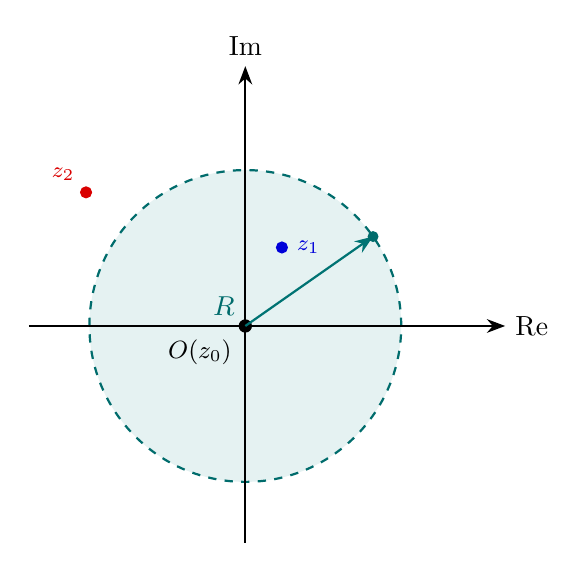
\begin{tikzpicture}[scale=1.1, >=Stealth]
    % 1. 底层：收敛圆内部着色与虚线边界（以原点 O 为展开中心 z_0）
    \fill[teal!10] (0, 0) circle (1.8cm);
    \draw[thick, dashed, teal!85!black] (0, 0) circle (1.8cm);

    % 2. 顶层：绘制贯穿且不被遮挡的坐标轴
    \draw[->, thick] (-2.5, 0) -- (3.0, 0) node[right] {$\operatorname{Re}$};
    \draw[->, thick] (0, -2.5) -- (0, 3.0) node[above] {$\operatorname{Im}$};

    % 3. 中心点 z_0 与原点 O
    \filldraw[black] (0, 0) circle (2pt);
    \node[below left=2pt, font=\small] at (0, 0) {$O (z_0)$};

    % 4. 收敛半径 R 箭头与圆周接触点
    \coordinate (Bpt) at (35:1.8cm);
    \draw[->, thick, teal!90!black] (0, 0) -- (Bpt);
    \node[teal!85!black, font=\small, midway, above left] at ($(0,0)!0.5!(Bpt)$) {$R$};
    \filldraw[teal!85!black] (Bpt) circle (1.6pt);

    % 5. 内部收敛点 z_1 与外部发散点 z_2（远离轴线）
    \coordinate (Z1) at (65:1.0cm);
    \filldraw[blue!85!black] (Z1) circle (1.8pt) node[right=2pt, font=\footnotesize] {$z_1$};

    \coordinate (Z2) at (140:2.4cm);
    \filldraw[red!85!black] (Z2) circle (1.8pt) node[above left=1pt, font=\footnotesize] {$z_2$};
\end{tikzpicture}
\caption{幂级数的收敛圆结构（圆盘内部 $|z - z_0| < R$ 处处绝对收敛；圆盘外部 $|z - z_0| > R$ 处处发散；圆周上至少存在一个和函数的奇点）}
\label{fig:convergence_circle}
\end{figure}

\begin{property}[和函数的解析性质]
设幂级数 $f(z) = \sum_{n=0}^\infty c_n (z - z_0)^n$ 的收敛半径为 $R > 0$，则：
\begin{enumerate}
    \item $f(z)$ 在开收敛圆盘 $|z - z_0| < R$ 内为\textbf{解析函数}；
    \item 幂级数在收敛圆内可\textbf{逐项求导}任意次，收敛半径保持不变，且
    \begin{equation}
        f'(z) = \sum_{n=1}^\infty n c_n (z - z_0)^{n-1}
    \end{equation}
    \item 幂级数沿收敛圆内任意连续曲线 $C$ 可\textbf{逐项积分}，且
    \begin{equation}
        \int_C f(z)\,\mathrm{d}z = \sum_{n=0}^\infty c_n \int_C (z - z_0)^n\,\mathrm{d}z
    \end{equation}
\end{enumerate}
\end{property}

\subsection{泰勒（Taylor）级数}

\begin{theorem}[泰勒展开定理]
设函数 $f(z)$ 在区域 $D$ 内解析。对于 $D$ 内任意一点 $z_0$，只要圆域 $K: |z - z_0| < R$ 完全包含于 $D$ 内，则 $f(z)$ 在该圆域内必能展开为唯一的幂级数：
\begin{equation}
    f(z) = \sum_{n=0}^\infty c_n (z - z_0)^n
\end{equation}
其展开系数由柯西积分或高阶导数唯一确定：
\begin{equation}
    c_n = \frac{1}{2\pi i} \oint_{|\zeta - z_0| = \rho} \frac{f(\zeta)}{(\zeta - z_0)^{n+1}}\,\mathrm{d}\zeta = \frac{f^{(n)}(z_0)}{n!} \qquad (n = 0, 1, 2, \dots)
\end{equation}
其中展开半径 $R$ 恰好等于展开中心 $z_0$ 到函数 $f(z)$ 距离最近的奇点之间的几何距离。
\end{theorem}

\begin{figure}[htbp]
\centering
\begin{tikzpicture}[scale=1.1, >=Stealth]
    % 解析区域 D
    \draw[thick, fill=blue!5, rounded corners=18pt] (-2.8, -2.0) rectangle (3.2, 2.0);
    \node[blue!80!black, font=\bfseries] at (2.6, 1.6) {$D$};

    % 中心点 z0 与展开圆 K
    \coordinate (Z0) at (-0.2, 0);
    \filldraw[black] (Z0) circle (2pt) node[below=3pt] {$z_0$};

    \draw[thick, dashed, blue!70!black] (Z0) circle (1.5cm);
    \draw[->, thick, blue!85!black] (Z0) -- ++(40:1.5cm) coordinate (Rpt);
    \node[blue!85!black, font=\small, midway, above left] at ($(Z0)!0.5!(Rpt)$) {$R$};

    % 最近奇点与边界
    \coordinate (Sing) at ($(Z0)+(40:1.5cm)$);
    \filldraw[red!85!black] (Sing) circle (2.2pt) node[right=3pt, red!85!black, font=\small] {$z_*$ (最近奇点)};

    % 圆周上的积分点与内部观测点
    \coordinate (Zpos) at ($(Z0)+(120:0.9cm)$);
    \filldraw[purple] (Zpos) circle (1.8pt) node[above right=1pt, font=\footnotesize] {$z$};

    \coordinate (Zeta) at ($(Z0)+(160:1.5cm)$);
    \filldraw[teal!85!black] (Zeta) circle (1.8pt) node[above left=1pt, font=\footnotesize] {$\zeta \in K$};
\end{tikzpicture}
\caption{泰勒展开定理几何原理（展开圆盘以 $z_0$ 到最近奇点 $z_*$ 的欧氏距离 $R = |z_* - z_0|$ 为最大半径；柯西核通过恒等式 $\frac{1}{\zeta - z} = \sum_{n=0}^\infty \frac{(z - z_0)^n}{(\zeta - z_0)^{n+1}}$ 展开）}
\label{fig:taylor_expansion}
\end{figure}

\begin{property}[常见初等函数的麦克劳林展开式]
在全复平面 $\mathbb{C}$ 上处处解析（$R = \infty$）的整函数展开式：
\begin{align}
    e^z &= \sum_{n=0}^\infty \frac{z^n}{n!} = 1 + z + \frac{z^2}{2!} + \frac{z^3}{3!} + \dots \\
    \sin z &= \sum_{n=0}^\infty \frac{(-1)^n}{(2n+1)!} z^{2n+1} = z - \frac{z^3}{3!} + \frac{z^5}{5!} - \dots \\
    \cos z &= \sum_{n=0}^\infty \frac{(-1)^n}{(2n)!} z^{2n} = 1 - \frac{z^2}{2!} + \frac{z^4}{4!} - \dots
\end{align}
在单位圆内（$R = 1$）解析的有理与对数函数主值展开式：
\begin{align}
    \frac{1}{1 - z} &= \sum_{n=0}^\infty z^n = 1 + z + z^2 + \dots \qquad (|z| < 1) \\
    \frac{1}{1 + z} &= \sum_{n=0}^\infty (-1)^n z^n = 1 - z + z^2 - \dots \qquad (|z| < 1) \\
    \ln(1 + z) &= \sum_{n=1}^\infty \frac{(-1)^{n-1}}{n} z^n = z - \frac{z^2}{2} + \frac{z^3}{3} - \dots \qquad (|z| < 1)
\end{align}
\end{property}

\subsection{洛朗（Laurent）级数}

\begin{definition}{双边幂级数}{laurent_series}
形如包含正负整数次幂的形式和
\begin{equation}
    \sum_{n=-\infty}^{+\infty} c_n (z - z_0)^n = \underbrace{\sum_{n=1}^\infty \frac{c_{-n}}{(z - z_0)^n}}_{\text{主要部分（负幂项）}} + \underbrace{\sum_{n=0}^\infty c_n (z - z_0)^n}_{\text{解析部分（正幂项）}}
\end{equation}
称为以 $z_0$ 为中心的\textbf{双边幂级数}或\textbf{洛朗级数}。
\end{definition}

\begin{theorem}[洛朗展开定理]
设函数 $f(z)$ 在圆环域 $D: R_1 < |z - z_0| < R_2$ ($0 \le R_1 < R_2 \le +\infty$) 内处处解析，则在该圆环域内，$f(z)$ 必能展开为唯一的双边幂级数：
\begin{equation}
    f(z) = \sum_{n=-\infty}^{+\infty} c_n (z - z_0)^n
\end{equation}
展开系数由环域内任意一条围绕中心 $z_0$ 的正向简单闭曲线 $C$ 的线积分给出：
\begin{equation}
    c_n = \frac{1}{2\pi i} \oint_C \frac{f(\zeta)}{(\zeta - z_0)^{n+1}}\,\mathrm{d}\zeta \qquad (n = 0, \pm 1, \pm 2, \dots)
\end{equation}
\end{theorem}

\begin{figure}[htbp]
\centering
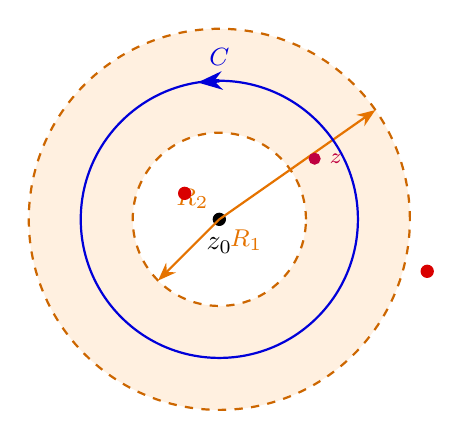
\begin{tikzpicture}[scale=1.1, >=Stealth]
    % 圆心
    \coordinate (Z0) at (0, 0);
    \filldraw[black] (Z0) circle (2pt) node[below=3pt] {$z_0$};

    % 圆环域底色 (R1=1.0, R2=2.2)
    \fill[orange!12, even odd rule] (Z0) circle (2.2cm) (Z0) circle (1.0cm);

    % 内外圆边界
    \draw[thick, dashed, orange!80!black] (Z0) circle (1.0cm);
    \draw[thick, dashed, orange!80!black] (Z0) circle (2.2cm);

    % 内外半径标注
    \draw[->, thick, orange!90!black] (Z0) -- ++(-135:1.0cm) coordinate (R1pt);
    \node[orange!90!black, font=\footnotesize, midway, below right] at ($(Z0)!0.5!(R1pt)$) {$R_1$};

    \draw[->, thick, orange!90!black] (Z0) -- ++(35:2.2cm) coordinate (R2pt);
    \node[orange!90!black, font=\footnotesize, midway, above left] at ($(Z0)!0.5!(R2pt)$) {$R_2$};

    % 环内封闭围道 C
    \draw[thick, blue!85!black] (Z0) circle (1.6cm);
    \draw[->, line width=1.3pt, blue!85!black] (0, 1.6) -- (-0.25, 1.58);
    \node[above=2pt, blue!85!black, font=\small] at (0, 1.6) {$C$};

    % 环内展开点 z
    \coordinate (Z) at (1.1, 0.7);
    \filldraw[purple] (Z) circle (1.8pt) node[right=2pt, font=\footnotesize] {$z$};

    % 内孔奇点与外域奇点
    \filldraw[red!85!black] (-0.4, 0.3) circle (2pt);
    \filldraw[red!85!black] (2.4, -0.6) circle (2pt);
\end{tikzpicture}
\caption{洛朗级数展开与圆环域几何模型（函数在同心圆环 $R_1 < |z - z_0| < R_2$ 内解析；内圆内部与外圆外部均可存在孤立奇点；闭围道 $C$ 在环内连续变形时不影响积分系数 $c_n$）}
\label{fig:laurent_ring}
\end{figure}

\begin{remark}
洛朗展开系数中的 $c_n$ 一般\textbf{不能}用微商表示为 $\frac{f^{(n)}(z_0)}{n!}$，因为在以 $z_0$ 为中心的整个实心圆盘内 $f(z)$ 往往含有奇点而不解析。

当 $n = -1$ 时，由洛朗展开系数公式可得：
\begin{equation}
    c_{-1} = \frac{1}{2\pi i} \oint_C f(z)\,\mathrm{d}z \iff \oint_C f(z)\,\mathrm{d}z = 2\pi i \cdot c_{-1}
\end{equation}
系数 $c_{-1}$ 直接关联闭围道积分，是后续第五章留数理论的核心基石。
\end{remark}

\section{留数}

\subsection{孤立奇点}

\begin{definition}{孤立奇点}{isolated_singularity}
设点 $z_0$ 为函数 $f(z)$ 的奇点。若存在某个去心邻域 $\mathring{U}(z_0, \delta) = \{z \in \mathbb{C} \mid 0 < |z - z_0| < \delta\}$，使得 $f(z)$ 在该去心邻域内处处解析，则称 $z_0$ 为 $f(z)$ 的\textbf{孤立奇点}。
\end{definition}

设 $f(z)$ 在去心圆环域 $0 < |z - z_0| < R$ 内展开为洛朗级数：
\begin{equation}
    f(z) = \sum_{n=-\infty}^{+\infty} c_n (z - z_0)^n = \sum_{n=1}^\infty \frac{c_{-n}}{(z - z_0)^n} + \sum_{n=0}^\infty c_n (z - z_0)^n
\end{equation}
根据其主要部分（负幂项部分）的构成，孤立奇点分为以下三类：
\begin{enumerate}
    \item \textbf{可去奇点}：主要部分完全为零（即无负幂项，$c_{-n} = 0, \forall n \ge 1$）。其等价刻画为：极限 $\lim_{z \to z_0} f(z) = c_0$ 存在且有限；或 $f(z)$ 在去心邻域内有界。
    \item \textbf{极点（$m$ 级极点）}：主要部分仅含有限个负幂项，且最高负幂为 $m$ 次（即 $c_{-m} \neq 0$ 且当 $n > m$ 时 $c_{-n} = 0$）。其等价刻画为：极限 $\lim_{z \to z_0} f(z) = \infty$。
    \item \textbf{本性奇点}：主要部分包含无穷多个负幂项。其等价刻画为：极限 $\lim_{z \to z_0} f(z)$ 既不存在也不为 $\infty$（Weierstrass 定理）。
\end{enumerate}

\begin{theorem}[零点与极点的对偶关系]
若 $z_0$ 是不恒为零的解析函数 $f(z)$ 的 $m$ 级零点（即 $f(z) = (z - z_0)^m \varphi(z)$ 且 $\varphi(z_0) \neq 0$），则 $z_0$ 必是亚纯函数 $\frac{1}{f(z)}$ 的 $m$ 级极点；反之，若 $z_0$ 为 $f(z)$ 的 $m$ 级极点，则 $z_0$ 必为 $\frac{1}{f(z)}$ 的 $m$ 级零点。
\end{theorem}

\subsection{留数的概念与留数定理}

\begin{definition}{留数}{residue}
设 $z_0$ 为函数 $f(z)$ 的孤立奇点，$C$ 为其去心解析邻域内围绕 $z_0$ 的任意一条正向简单闭曲线。称复常数
\begin{equation}
    \operatorname{Res}[f(z), z_0] = \frac{1}{2\pi i} \oint_C f(z)\,\mathrm{d}z
\end{equation}
为 $f(z)$ 在点 $z_0$ 处的\textbf{留数}（又记为 $\operatorname{Res}(f, z_0)$）。其数值恰等于 $f(z)$ 在点 $z_0$ 处洛朗级数展开中负一次方项的系数 $c_{-1}$。
\end{definition}

\begin{theorem}[柯西留数定理]
设闭区域 $\bar{D}$ 的外边界为简单正向闭曲线 $C$。若函数 $f(z)$ 在 $D$ 内除有限个孤立奇点 $z_1, z_2, \dots, z_n$ 外处处解析，且在闭边界 $C$ 上连续无奇点，则：
\begin{equation}
    \oint_C f(z)\,\mathrm{d}z = 2\pi i \sum_{k=1}^n \operatorname{Res}[f(z), z_k]
\end{equation}
\end{theorem}

\begin{figure}[htbp]
\centering
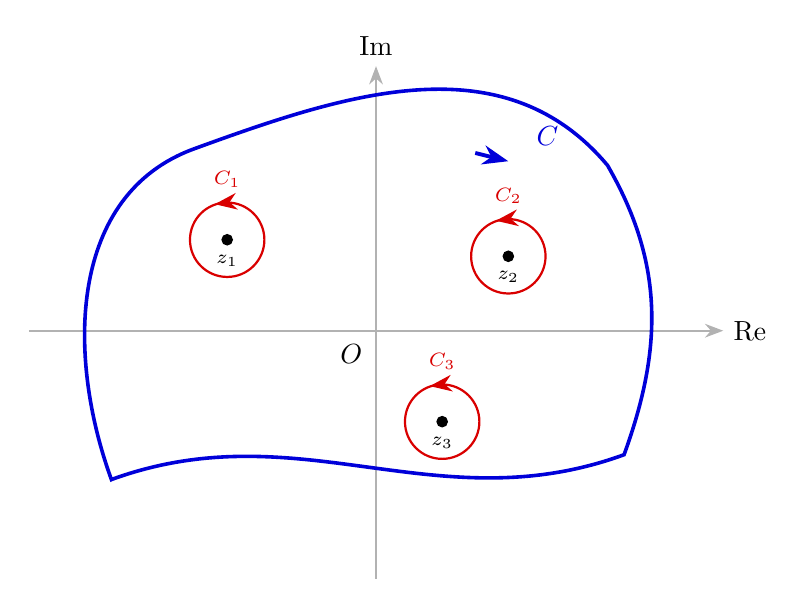
\begin{tikzpicture}[scale=1.05, >=Stealth]
    % 贯穿的底层坐标轴
    \draw[->, thick, gray!60] (-4.2, 0) -- (4.2, 0) node[right, black] {$\operatorname{Re}$};
    \draw[->, thick, gray!60] (0, -3.0) -- (0, 3.2) node[above, black] {$\operatorname{Im}$};
    \node[below left=2pt] at (0, 0) {$O$};

    % 外围闭路 C（形态开阔饱满，留足内部安全空间）
    \draw[line width=1.3pt, blue!85!black] 
        (-3.2, -1.8) to[out=20, in=200] (3.0, -1.5)
        to[out=70, in=300] (2.8, 2.0)
        to[out=130, in=20] (-2.2, 2.2)
        to[out=200, in=110] cycle;
    
    % 外闭路方向与标注（置于右上开阔外侧，不压轴线）
    \draw[->, line width=1.4pt, blue!85!black] (1.2, 2.15) -- (1.6, 2.05);
    \node[above right=1pt, blue!85!black, font=\bfseries] at (1.8, 2.1) {$C$};

    % 奇点 z1 及小圆周 C1（第二象限）
    \coordinate (Z1) at (-1.8, 1.1);
    \draw[thick, red!85!black] (Z1) circle (0.45cm);
    \draw[->, line width=1.1pt, red!85!black] (-1.8, 1.55) -- (-1.95, 1.53);
    \filldraw[black] (Z1) circle (1.8pt) node[below=2pt, font=\scriptsize] {$z_1$};
    \node[above=2pt, red!85!black, font=\scriptsize] at (-1.8, 1.55) {$C_1$};

    % 奇点 z2 及小圆周 C2（第一象限）
    \coordinate (Z2) at (1.6, 0.9);
    \draw[thick, red!85!black] (Z2) circle (0.45cm);
    \draw[->, line width=1.1pt, red!85!black] (1.6, 1.35) -- (1.45, 1.33);
    \filldraw[black] (Z2) circle (1.8pt) node[below=2pt, font=\scriptsize] {$z_2$};
    \node[above=2pt, red!85!black, font=\scriptsize] at (1.6, 1.35) {$C_2$};

    % 奇点 z3 及小圆周 C3（第四象限，远离边界与坐标轴）
    \coordinate (Z3) at (0.8, -1.1);
    \draw[thick, red!85!black] (Z3) circle (0.45cm);
    \draw[->, line width=1.1pt, red!85!black] (0.8, -0.65) -- (0.65, -0.67);
    \filldraw[black] (Z3) circle (1.8pt) node[below=2pt, font=\scriptsize] {$z_3$};
    \node[above=2pt, red!85!black, font=\scriptsize] at (0.8, -0.65) {$C_3$};
\end{tikzpicture}
\caption{柯西留数定理围道拓扑模型（外闭路线 $C$ 内部积分转化为围绕各独立奇点的小圆周 $C_k$ 留数之和，即 $\oint_C f(z)\,\mathrm{d}z = 2\pi i \sum_{k=1}^n \operatorname{Res}[f(z), z_k]$）}
\label{fig:residue_theorem}
\end{figure}

\begin{property}[极点留数计算规则]
\begin{enumerate}
    \item \textbf{规则 I（一级极点）}：若 $z_0$ 为 $f(z)$ 的一级极点，则：
    \begin{equation}
        \operatorname{Res}[f(z), z_0] = \lim_{z \to z_0} (z - z_0) f(z)
    \end{equation}
    \item \textbf{规则 II（$m$ 级极点）}：若 $z_0$ 为 $f(z)$ 的 $m$ 级极点，则：
    \begin{equation}
        \operatorname{Res}[f(z), z_0] = \frac{1}{(m - 1)!} \lim_{z \to z_0} \frac{\mathrm{d}^{m-1}}{\mathrm{d}z^{m-1}} \Big[ (z - z_0)^m f(z) \Big]
    \end{equation}
    \item \textbf{规则 III（分式型一级极点）}：设 $f(z) = \frac{P(z)}{Q(z)}$，其中 $P(z), Q(z)$ 在 $z_0$ 处解析。若 $P(z_0) \neq 0, Q(z_0) = 0$ 且 $Q'(z_0) \neq 0$，则：
    \begin{equation}
        \operatorname{Res}[f(z), z_0] = \frac{P(z_0)}{Q'(z_0)}
    \end{equation}
\end{enumerate}
\end{property}

\subsection{无穷远点处的留数}

\begin{definition}{无穷远点的留数}{residue_at_infinity}
设无穷远点 $z = \infty$ 是函数 $f(z)$ 的孤立奇点（即在圆环域 $R < |z| < +\infty$ 内解析），取包含原点及一切有限奇点的圆周 $C: |z| = \rho > R$，定义 $f(z)$ 在 $\infty$ 处的\textbf{留数为沿 $C$ 顺时针（负向 $C^-$）的积分值}：
\begin{equation}
    \operatorname{Res}[f(z), \infty] = \frac{1}{2\pi i} \oint_{C^-} f(z)\,\mathrm{d}z = -\frac{1}{2\pi i} \oint_C f(z)\,\mathrm{d}z
\end{equation}
若 $f(z)$ 在圆环域内的洛朗展开式为 $f(z) = \sum_{n=-\infty}^{+\infty} c_n z^n$，则 $\operatorname{Res}[f(z), \infty] = -c_{-1}$。
\end{definition}

\begin{theorem}[全平面留数总和定理]
若函数 $f(z)$ 在扩充复平面 $\bar{\mathbb{C}}$ 上除有限个孤立奇点 $z_1, z_2, \dots, z_n$ 及 $\infty$ 外处处解析，则其在全平面所有奇点处的留数总和恒为零：
\begin{equation}
    \operatorname{Res}[f(z), \infty] + \sum_{k=1}^n \operatorname{Res}[f(z), z_k] = 0
\end{equation}
\end{theorem}

\begin{property}[无穷远点留数的代换求法]
作变换 $z = \frac{1}{t}$，可将无穷远点的留数化为原点处的有限留数计算：
\begin{equation}
    \operatorname{Res}[f(z), \infty] = -\operatorname{Res}\left[ f\left(\frac{1}{t}\right)\frac{1}{t^2},\, 0 \right]
\end{equation}
\end{property}

\subsection{留数在计算实积分中的应用}

\subsubsection{三角有理式定积分}
计算积分 $\int_0^{2\pi} R(\cos\theta, \sin\theta)\,\mathrm{d}\theta$。令 $z = e^{i\theta}$（$0 \le \theta \le 2\pi$），对应正向单位圆周 $C: |z| = 1$。利用代换：
\begin{equation}
    \cos\theta = \frac{z + z^{-1}}{2}, \qquad \sin\theta = \frac{z - z^{-1}}{2i}, \qquad \mathrm{d}\theta = \frac{\mathrm{d}z}{iz}
\end{equation}
原积分转化为单位圆周内的复回路积分：
\begin{equation}
    \int_0^{2\pi} R(\cos\theta, \sin\theta)\,\mathrm{d}\theta = \oint_{|z|=1} R\left(\frac{z+z^{-1}}{2}, \frac{z-z^{-1}}{2i}\right)\frac{\mathrm{d}z}{iz} = 2\pi i \sum_{|z_k|<1} \operatorname{Res}[f(z), z_k]
\end{equation}

\subsubsection{实轴有理函数的无穷反常积分}
计算积分 $\int_{-\infty}^{+\infty} \frac{P(x)}{Q(x)}\,\mathrm{d}x$。设 $Q(x)$ 在实轴上无实零点，且分母次数比分子次数至少高二次（$\deg Q \ge \deg P + 2$）。选取由实轴截段 $[-R, R]$ 与上半平面大圆弧 $C_R: z = R e^{i\theta}$ ($0 \le \theta \le \pi$) 构成的闭积分围道。

当 $R \to \infty$ 时，根据估值定理 $\lim_{R \to \infty} \int_{C_R} \frac{P(z)}{Q(z)}\,\mathrm{d}z = 0$，由此得到：
\begin{equation}
    \int_{-\infty}^{+\infty} \frac{P(x)}{Q(x)}\,\mathrm{d}x = 2\pi i \sum_{\operatorname{Im}(z_k) > 0} \operatorname{Res}\left[\frac{P(z)}{Q(z)},\, z_k\right]
\end{equation}

\subsubsection{含三角因子的傅里叶型积分与若尔当（Jordan）引理}
\begin{lemma}[若尔当引理]
设函数 $g(z)$ 在上半平面 $|z| \ge R_0, \operatorname{Im}(z) \ge 0$ 上连续，且当 $z \to \infty$ 时关于 $\arg z$ 一致趋于零（即 $M(R) = \max_{C_R} |g(z)| \to 0, R \to \infty$）。若 $m > 0$，则：
\begin{equation}
    \lim_{R \to \infty} \int_{C_R} g(z) e^{imz}\,\mathrm{d}z = 0
\end{equation}
\end{lemma}

利用欧拉公式 $\cos(mx) = \operatorname{Re}(e^{imx}), \sin(mx) = \operatorname{Im}(e^{imx})$，可将实积分转化为含指数因子的复积分计算：
\begin{equation}
    \int_{-\infty}^{+\infty} g(x)\cos(mx)\,\mathrm{d}x = \operatorname{Re}\left( 2\pi i \sum_{\operatorname{Im}(z_k) > 0} \operatorname{Res}[g(z)e^{imz}, z_k] \right)
\end{equation}

\subsection{对数留数与辐角原理}

\begin{theorem}[对数留数定理]
设 $C$ 为正向简单闭曲线。若函数 $f(z)$ 在 $C$ 上解析且不为零，在 $C$ 内部除有限个极点外处处解析，则：
\begin{equation}
    \frac{1}{2\pi i} \oint_C \frac{f'(z)}{f(z)}\,\mathrm{d}z = N - P
\end{equation}
其中 $N$ 为 $f(z)$ 在 $C$ 内部零点的总个数（重数计入），$P$ 为 $f(z)$ 在 $C$ 内部极点的总个数（阶数计入）。
\end{theorem}

\begin{theorem}[辐角原理]
在对数留数定理的条件下，记 $z$ 沿曲线 $C$ 正向绕行一周时函数值 $f(z)$ 的总辐角改变值为 $\Delta_C \operatorname{Arg} f(z)$，则：
\begin{equation}
    N - P = \frac{1}{2\pi} \Delta_C \operatorname{Arg} f(z)
\end{equation}
几何上，$\frac{1}{2\pi}\Delta_C \operatorname{Arg} f(z)$ 正是 $z$ 沿 $C$ 绕行一周时，象曲线 $\Gamma = f(C)$ 围绕 $w$ 平面原点逆时针旋转的总转数。
\end{theorem}

\begin{figure}[htbp]
\centering
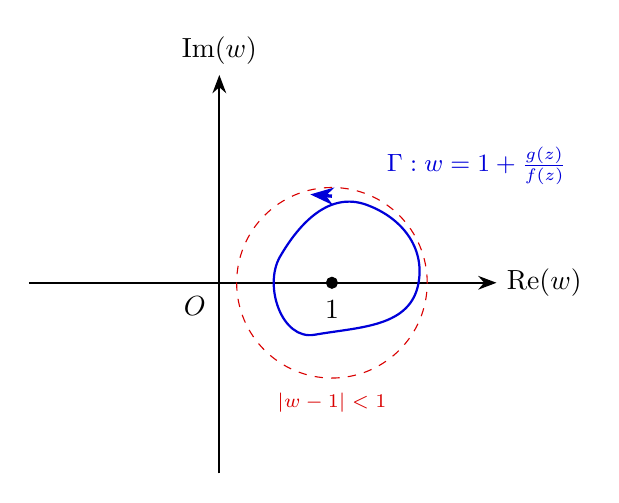
\begin{tikzpicture}[scale=1.1, >=Stealth]
    % 贯穿坐标轴
    \draw[->, thick] (-2.2, 0) -- (3.2, 0) node[right] {$\operatorname{Re}(w)$};
    \draw[->, thick] (0, -2.2) -- (0, 2.4) node[above] {$\operatorname{Im}(w)$};
    \node[below left=2pt] at (0, 0) {$O$};

    % 原点与基准点 1
    \filldraw[black] (1.3, 0) circle (1.8pt) node[below=3pt] {$1$};

    % 围绕 1 的象曲线 Gamma (以 1 为中心扰动)
    \draw[thick, blue!85!black] (1.3, 0) ++(0:1.0cm) to[out=80, in=-20] ++(-0.6, 0.9)
        to[out=160, in=60] ++(-1.0, -0.6) to[out=240, in=190] ++(0.4, -0.9)
        to[out=10, in=260] cycle;
    \draw[->, line width=1.2pt, blue!85!black] (1.3, 1.0) -- (1.05, 1.02);
    \node[above right=1pt, blue!85!black, font=\small] at (1.8, 1.0) {$\Gamma: w = 1 + \frac{g(z)}{f(z)}$};

    % 单位圆盘围绕 1，且不包含原点 O
    \draw[dashed, red!85!black] (1.3, 0) circle (1.1cm);
    \node[below=2pt, red!85!black, font=\scriptsize] at (1.3, -1.1) {$|w - 1| < 1$};
\end{tikzpicture}
\caption{路西定理象曲线模型（条件 $|g(z)| < |f(z)|$ 保证象曲线 $\Gamma$ 始终落在以 1 为中心、半径小于 1 的圆盘内；曲线不包围原点，故关于原点的辐角改变量恒为零）}
\label{fig:rouche_theorem}
\end{figure}

\begin{theorem}[路西（Rouché）定理]
设 $C$ 为正向简单闭曲线。若函数 $f(z)$ 和 $g(z)$ 在闭曲线 $C$ 及其内部均解析，且在边界 $C$ 上处处满足严格不等式：
\begin{equation}
    |g(z)| < |f(z)|
\end{equation}
则函数 $f(z)$ 与 $f(z) + g(z)$ 在闭曲线 $C$ 的内部具有相同数目的零点（计入重数）。
\end{theorem}

\end{document}